\documentclass[ams]{U-AizuGT}


\usepackage{pifont}
%\usepackage[dvipdfmx]{graphicx}
\usepackage{graphicx}
\usepackage{cite}
\usepackage{algorithm}
\usepackage{algpseudocode}
\usepackage{subcaption}
\usepackage{amsmath}


%% Macro
\def\x{\mathbf{x}}
\def\R{\mathbb{R}}
\def\n{\mathbf{n}}
\def\bbeta{\boldsymbol\beta}
%%


\author{Shingo Ito}
\studentid{1200045}
\supervisor{Pierre-Alain Fayolle}

\title{A simple approach to mesh deformation}


\begin{document}

\maketitle

\begin{abstract}
In this dissertation, we present a simple approach for mesh deformation. 
Points are sampled from the surface represented by the triangle mesh. 
The point cloud data is deformed instead of the mesh. 
A surface reconstruction algorithm is finally used to reconstruct the surface from the deformed point cloud, preventing defects usually appearing in mesh deformation algorithms.
\end{abstract}


\section*{Keywords:}
Mesh processing; Mesh deformation; Surface reconstruction


\section{Introduction}
Mesh processing and mesh deformation is an important research topic in the geometric modeling community, with important practical applications. It allows users with relatively little technical knowledge to model complex freeform shapes through simple and intuitive interfaces. Shape deformation is a challenging topic because it can require complex mathematical formulations to be implemented as efficient (in terms of speed) computer programs.
The topic of shape deformation and shape sculpture is a popular topic in geometric modeling. See for example \cite{BKPAL10} for a survey of recent mesh-based deformation approaches. One of the problems with the typical mesh-based deformation approaches is that they may lead to defects in the input triangle mesh, such as self-intersection for example. In order to overcome this difficulty, we propose an algorithm where a sampling of the triangle mesh is deformed and the deformed surface is obtained from applying a surface reconstruction algorithm to the deformed point cloud. Our deformation algorithm works by applying a vector field, corresponding to the deformation, to the vertices of a triangle mesh. In order to prevent defects in the mesh such as self-intersection, we reconstruct a surface from the deformed vertices by using a standard surface reconstruction algorithm.


\section{Related works}
Surface deformation is an important research topic in shape and geometric modeling. 
The book by Botsch and colleagues on polygon mesh processing \cite{BKPAL10} has a full 
chapter on techniques for polygon mesh deformation and provides many related references on the topic. 
When surfaces are represented implicitly, the main technique consists in computing an 
approximation of the distance to the zero level-set and deforming this distance field. 
The dissertation of Bridson \cite{B03} describes such a technique. 
More recently the dissertation of Jacobson \cite{J13} presents various novel techniques 
for mesh deformation techniques based on variational methods and solving partial differential equations. 
It also contains several references related to the domain of mesh deformation.


\section{Algorithm}
\label{algorithm}
Algorithms for surface deformation traditionally work by moving the triangle mesh vertices according to some specified vector field corresponding to the deformation. Depending on how the deformation is computed, this approach can result in defects in the triangle mesh such as for example self-intersecting triangles. In this work we propose to apply the deformation to a sampling of the surface and reconstruct the deformed surface by using a surface reconstruction algorithm. Our approach is summarized in the algorithm \ref{alg:main} below.

\begin{algorithm}
\caption{Overview of the main approach}
\label{alg:main}
\begin{algorithmic}
\State{Sample from the surface}
\State{Apply the deformation field to the samples}
\State{Apply a surface reconstruction algorithm to the samples}
\end{algorithmic}
\end{algorithm}


\subsection{Surface sampling}
The input surface is represented by a triangle mesh read from a file. 
If the triangle mesh is dense enough, we select as points the mesh vertices. 
Otherwise we uniformly sample from each triangle according to the following method \ref{alg:sample}.

\begin{algorithm}
\caption{Uniform sampling from a triangle}
\label{alg:sample}
\begin{algorithmic}
\Function{Sample}{$p_1$, $p_2$, $p_3$, $\xi_1$, $\xi_2$}

\Comment{$p_1$, $p_2$ and $p_3$ are the triangle vertices, 
$\xi_1$ and $\xi_2$ are samples from a uniform distribution}

\State Compute the barycentric coordinates: $u = 1-\sqrt{\xi_1}$ 
and $v = \xi_2 \sqrt{\xi_1}$
\State Compute the sample: $P = u * p_1 + v * p_2 + (1 - u - v) * p_3$

\Return $P$
\EndFunction
\end{algorithmic}
\end{algorithm}
  

\subsection{Points deformation}
There are different possible approaches for deforming points. We have implemented the following simple approach.
Given a selected vertex from the input surface, we displace each point in the normal direction
by a truncated Gaussian centered on this selected vertex:
\[
f(\x)=
\begin{cases}
\frac{1}{\sqrt{2\pi\sigma^2}} \exp\left(- \frac{(\x- \x_S)^{2}}{2 \sigma^{2}}\right) & \text{if } \|\x-\x_S\| < r \\
0 & \text{otherwise}
\end{cases}
\]
In this expression, $x_S$ is the selected vertex, $\sigma$ controls the width of the Gaussian and $r$ controls 
the radius of support of the truncated Gaussian.

After deformation, we need to recompute the normal vector to each point of the point cloud 
since it is needed for the surface reconstruction algorithms described in the next section.
We used the implementation provided by CGAL \cite{cgal} for normal computation and orientation.
It implements the algorithm described in \cite{HRDMS92}.

\subsection{Surface reconstruction}
Given the deformed point-cloud, we then apply a surface reconstruction algorithm to reconstruct a surface from it. 
We have implemented and experimented with three surface reconstruction algorithms in our implementation.
All approaches are implicit surface based surface reconstruction algorithms. 
It means that the surface is obtained as the zero level-set of a function $f: \R^3 \rightarrow \R$. 

\paragraph{Hermite Radial Basis Functions}
First we have implemented Hermite Radial Basis Functions surface reconstruction (HRBF) 
surface reconstruction \cite{MGV11}. 
Given a set of points $P = {\x_i}$ with normal vector at each point $N = {\n_i}$, 
the output of the method is a function: $f : \R^3 \to \R$ defined as follows:
\[
f(\x)=\sum_{i=1}^n(\alpha_i\phi(\|\x-\x_i\|)-\bbeta_i\nabla\phi(\|\x-\x_i\|))
\]
where $\phi$ is a radially symmetric functions (compactly supported or not), 
%$\phi(t) = t^3$  and 
$\alpha_i \in \R$ and $\beta_i \in \R^3$ are unknown coefficients to be determined. 
The conditions used to determine the coefficients are: \[f(\x_i) = 0, \x_i \in \R^3\]
for interpolating points on the surface. And: \[\nabla f(\x_i)=\n_i, \x_i \in \R^3, \n_i \in \R^3\]
for interpolating the normals on the surface.
Taking into account the expression of $f$, we have:
\[f(\x_i)=\sum_{j=1}^n(\alpha_j\phi(\|\x_i-\x_j\|)-\bbeta_j\nabla\phi(\|\x_i-\x_j\|))=0\]
and
\[\nabla f(\x_i)=\sum_{j=1}^n(\alpha_j\nabla\phi(\|\x_i-\x_j\|)-H\phi(\|\x_i-\x_j\|)\bbeta_j)=\n_i\]
where $H$ is the Hessian matrix of $\phi$.
\\
The interpolation conditions can be written as:
%\[
\begin{align} \label{hrbf1}
 & \sum_{j=1}^n
\begin{bmatrix}
\phi(\|\x_i-\x_j\|) & -\nabla\phi(\|\x_i-\x_j\|)^T\\ \nabla\phi(\|\x_i-\x_j\|) & -H\phi(\|\x_i-\x_j\|)
\end{bmatrix}
\begin{bmatrix}
\alpha_j\\\bbeta_j
\end{bmatrix} \nonumber
\\
 & + \sum_{l=1}^m\lambda_l
\begin{bmatrix}
p_l(\x_i)\\\nabla p_l(\x_i)
\end{bmatrix}
=
\begin{bmatrix}
0 \\ \n_i
\end{bmatrix}
\end{align}
%\]
With the additional condition:
\begin{equation} \label{hrbfcond}
\sum_{j=1}^n[p_k(x_j)\nabla p_k(x_j)^T]\begin{bmatrix}\alpha_j\\\bbeta_j\end{bmatrix}=0
\end{equation}

Popular choices of radial basis function are: 
$\phi(\|x\|) = \|x\|$ or $\phi(\|x\|) = \|x\|^3$ or Wendland's compactly supported functions.
In our experiments we have implemented: $\phi(\|x\|) = \|x\|^3$.
Gradient and Hessian matrix of $\phi$ are given by:
\[\nabla\phi(\|x\|) = 3x\|x\|\]
\[ H \phi (\|x\|)= \left\{ \begin{array}{ll} 3/\|x\|(\|x\|^2I_{3\times3}) + xx^T, & \|x\| \neq 0\\ 
0_{3\times3}, &\|x\| = 0 \end{array}\right.\]
where $I_{3\times3}$ is the identity matrix and $0_{3\times3}$ is the zero matrix.

The system of linear equations in (\ref{hrbf1}) with the conditions (\ref{hrbfcond}) can be 
rewritten in matrix form as:
$\mathbf{A} \mathbf{w} = \mathbf{b}$
where the vector $\mathbf{w}$ contains the unknown coefficients. 
They are obtained from inverting the matrix $\mathbf{A}$.

\paragraph{Closed form approximation for compactly supported functions}
The use of non-compactly supported splines results in a dense matrix, 
which makes the approach above not practical for large point sets.
In order to handle such large point sets, it is preferrable to use 
compactly supported basis functions such as the ones proposed 
by Wendland \cite{MGV11}. 
In a recent work, Liu and Wang \cite{LW15} showed that when Wendland's 
compactly supported radial basis functions are used in the approach above, 
it is possible to obtain a good approximation to the solution in closed form.
Most notably their approach does not involve solving any linear system.
In their approach, the implicit surface is obtained from the function:  
\begin{equation} \label{hrbfclosed}
f(x)=-\sum_{j=1}^n<\frac{\rho^2_j}{20+\eta\rho^2_j} \n_j, \nabla\phi_{\rho_j}(\|\x-\x_j\|)>
\end{equation}
where $\rho_j$ is the radius of support of the basis function associated to the center $j$, 
and $\phi$ is the compactly supported basis function. 
In this paper, we use one of the Wendland's CSRBF \cite{WP95}: 
\[
\phi_{\rho}(r)=\phi(r/\rho)
\]
where:
\[
\phi (t)= \left\{ \begin{array}{ll} (1-t)^{4}(4t+1), & t \in [0,1]\\ 
0, & \text{otherwise} \end{array}\right.
\]
and $r$ is the Euclidean distance between the query point $\x$ and one of 
the centers.
In our experiments below, we use a constant $\rho$ given by 
the average spacing between the $6$ nearest neighbors and a given point 
of the input point-set. 

\paragraph{Poisson surface reconstruction}
\label{Poisson_recon}
The last surface reconstruction algorithm that we experimented with is 
the Poisson surface reconstruction \cite{KBH06}.
For our experiments, we used the implementation provided 
by CGAL \cite{cgal}.
This algorithm works by computing an indicator function $f$ for the solid 
to be reconstructed. An indicator function $f_S$ for a given solid $S$ is 
a function, such that: $f_S(\x) = 1$ for $\x \in S$ and $f_S(\x) = 0$ otherwise. 
In the case of the Poisson surface reconstruction approach, the indicator function
$f$ is obtained by solving the Poisson equation:
\begin{equation}\label{Poisson_eq}
\Delta f=div(\n)
\end{equation}
where $\n$ is an extrapolation of the given normal vector field.
The CGAL implementation solves (\ref{Poisson_eq}) with 
the finite element method on a tetrahedral mesh. 
This mesh is obtained from computing the refined Delaunay tetrahedralization 
of an enlarged bounding box of the input point-cloud.
Piecewise linear basis functions are used in the finite element method. 


\subsection{Implicit surface meshing}
In order to obtain a deformed surface, we need to compute a triangle mesh implementation of 
the implicit surface computed as described in the previous section. 

\paragraph{Marching Cubes}
The most common technique for meshing the zero level-set of implicit surface relies 
on the Marching Cubes algorithm \cite{LC87}.
The Marching Cubes algorithm is an algorithm for rendering isosurfaces from volumetric data. 
The basic idea is to consider a bounding box for the object to be meshed and subdivide it 
regularly into smaller cells
Then the function $f$ is sampled at the eight corners of each cell. 
If one or more values is less than the user-specified isovalue, and one or more have values 
is greater than this isovalue, the cell must intersect the isosurface.
By determining the edges in the cell that are intersected by the isosurface, 
and connecting them we can form a linear approximation of the surface in each cell.
By connecting the patches from all cells, we get a linear approximation of the isosurface.

\paragraph{Delaunay based implicit surface meshing}
\label{Delaunay_mesh}
Since we know that all the points from the deformed point-cloud belong to the surface 
of the deformed object (or at least are close to it), 
Marching Cubes based algorithm do not look like the most effective approach.
Instead one could compute a Delaunay tetrahedralization of the deformed point-cloud and peel off outside 
tetrahedra using the fitted function (either from the HRBF or Poisson surface reconstruction approach).
One practical implementation is the implicit surface mesh generator implemented by CGAL
which is an implementation of the algorithm of Boissonat and Oudot \cite{BO05}.


\section{Experiments and results}
A prototype for the methods described in section \ref{algorithm} was implemented on a laptop
with the following specifications: CPU is 1.4GHz Intel Core i5, Memory is 4 GB 1600 MHz DDR3, 
graphics board is Intel HD Graphics 5000 1536 MB, 
OS is OS X Yosemite version 10.10.5. 
It was implemented in C++ using the following libraries: CGAL4.7, OpenGL and Eigen.


\subsection{Deformation of a sphere}

\begin{figure*}
\hbox{
\centering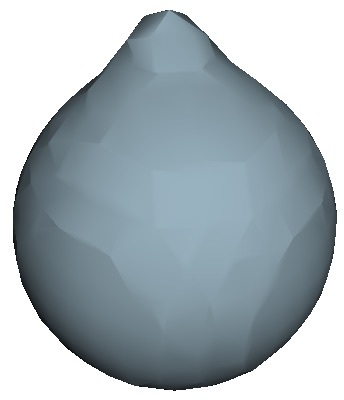
\includegraphics[width=0.3\textwidth]{deformed_sphere_hrbf.jpg}
\centering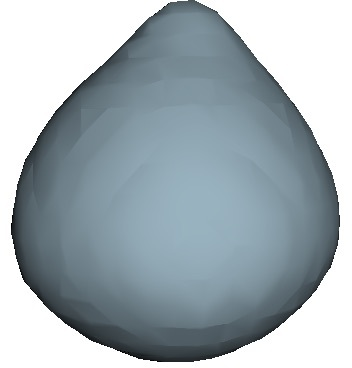
\includegraphics[width=0.3\textwidth]{deformed_sphere_hrbfclosed-3.jpg}
\centering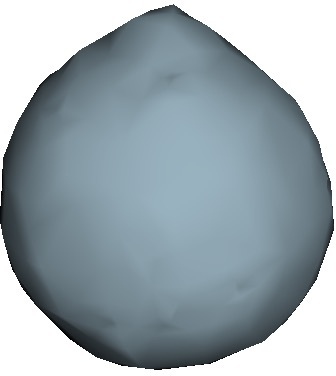
\includegraphics[width=0.3\textwidth]{deformed_sphere_poisson.jpg}
}
\caption{Deformed sphere using (from left to right): the HRBF approach, 
the closed form solution to the HRBF approach and the Poisson surface
reconstruction approach} \label{fig:sphere}
\end{figure*}

In the first experiment, we start from a sphere represented by a triangle mesh, 
made of 174 vertices and 344 triangles. The algorithm \ref{algorithm} is applied to 
deform the sphere. Figure \ref{fig:sphere} shows, from left to right,  
the results obtained with respectively: the HRBF reconstruction approach with 
the basis function $\|x\|^3$, the closed form approximation (\ref{hrbfclosed}) 
to the HRBF approach when compactly supported splines are used 
and the Poisson surface reconstrion approach.

%\begin{figure}
%  \centering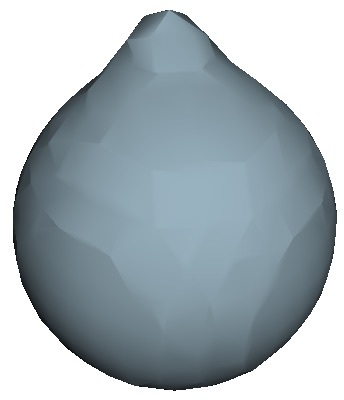
\includegraphics[width=0.7\columnwidth]{deformed_sphere_hrbf.jpg}
%  \caption{Deformed sphere using the HRBF approach} \label{fig:hrbf}
%\end{figure}
% 
%\begin{figure}
%  \centering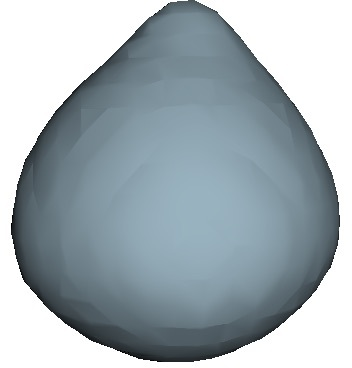
\includegraphics[width=0.7\columnwidth]{deformed_sphere_hrbfclosed-3.jpg}
%  \caption{Deformed sphere using the closed form solution to the HRBF approach} \label{fig:closed}
%\end{figure}
%
%\begin{figure}
%  \centering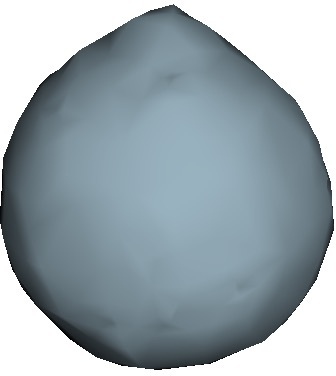
\includegraphics[width=0.7\columnwidth]{deformed_sphere_poisson.jpg}
%  \caption{Deformed sphere using the Poisson surface reconstruction approach} \label{fig:Poisson}
%\end{figure}
In our experiments, HRBF with the basis function $\|x\|^3$ is giving the best result 
but it is also the slowest approach. 
Additionally, it takes too much memory when non-compactly supported splines are used, 
because it needs to store a dense matrix in memory.
It makes the approach impractical for large triangle meshes. 
The closed form approximation to HRBF is faster but in our experiments 
we found it a bit difficult to control its behavior.
Poisson surface reconstruction is fast enough and results in accurate enough reconstructed surfaces. 
However, it tends to produce smoother surface. For example observe the difference between
the left and right images in fig. \ref{fig:sphere}.

\subsection{Example of sculpture}
\begin{figure}
  \centering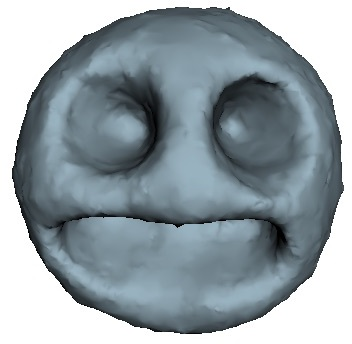
\includegraphics[width=0.7\columnwidth]{simple_face_poisson-2.jpg}
  \caption{Example to model a simple character face} \label{fig:face}
\end{figure}
Starting from a simple sphere, we used our program to model a simple character face. 
The result is illustrated in fig. \ref{fig:face}.
The eyes and the mouth were carved by changing the sign of the field 
used for the deformation. 
In addition, changing the width of the Gaussian function used for the deformation 
could allow to add or carve smaller details.

\subsection{Deformation of a more complex surface}
\begin{figure}
  \centering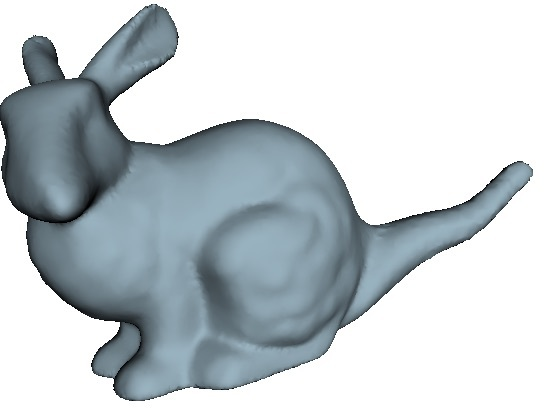
\includegraphics[width=0.7\columnwidth]{deformed_bunny_poisson.jpg}
  \caption{Deformed bunny object with stretched tail and nose} \label{fig:bunnyPoisson}
\end{figure}
%\begin{figure}
% \centering\includegraphics[width=0.7\columnwidth]{deformed_bunny_hrbfclosed.jpg}
% \caption{Deformed tail of bunny} \label{fig:bunnyHrbfclosed}
%\end{figure}
Figure \ref{fig:bunnyPoisson} illustrates the result of the deformation of a more complex
input mesh: the Stanford bunny.
The input mesh for this object contains 14072 vertices and 28042 triangles.
The Poisson surface reconstruction approach (see section \ref{Poisson_recon}) 
and Delaunay based meshing (see section \ref{Delaunay_mesh}) are used.
In this example, both the tail and the nose are stretched.

\subsection{Recommendations}
Based on our experiments, we recommend to use the HRBF approach 
with a non-compact basis function for small mesh (mesh with few vertices), 
and the Poisson based approach for larger mesh (mesh with a large number of vertices). 
It seems preferrable to mesh the implicit surface using the Delaunay based 
approach since it will keep existing points (original and deformed mesh vertices).
And therefore will better preserve details without sacrifying too much in term of performance. 


\section{Conclusion}
In this paper, we proposed a simple algorithm for mesh deformation that works by applying a deformation field to the vertices (or a sampling) of a triangle mesh and reconstructs the deformed surface from the deformed point-cloud.
Reconstruction from the point-cloud is made by fitting an implicit surface to the point-cloud and meshing it.
Different algorithms for implicit surface fitting were experimented. 
We used our prototype for creating simple deformations of triangle meshes and simple sculptures. 

Our algorithm and its implementation can be improved in several ways. This is left for future works.
Some examples of possible improvement include:  
implementing parts of the algorithm on the graphics card (GPU), using a modified meshing algorithm that tracks the surface, and exploiting the locality of the deformation. 
%%\\
%%The first way to improve the efficiency of our approach is to implement the algorithm for fitting and evaluating the RBF as well as the meshing algorithm (the Marching Cubes) on the graphics card. One of the bottleneck of the current algorithm is the evaluation of the fitted function on the corners of every cell in the regular grid used by the Marching Cubes algorithm. It is possible to improve this approach by considering only the grid cells near the surface (this information is provided by the deformed point-cloud). 
%%\\
%%When compactly supported splines (the spline is non-zero on a compact set) are used in the HRBF approach(Closed HRBF), it does not seem necessary to recompute the function value at cells corners away from the deformed region. This should allow to further decrease the computational time when multiple deformations are applied on a given object.


\section*{Acknowledgement}
The bunny model is courtesy of the Stanford Computer Graphics Laboratory.


\bibliographystyle{ieice}
\bibliography{s1200045}


\end{document}
